\documentclass[svgnames,11pt]{beamer}
\setbeamercolor{structure}{fg=SlateGray}
\usetheme{Goettingen}
\input{/home/tof/Documents/Cozy/latex-include/preambule_commun.tex}
\usepackage{pgfpages}
\setbeameroption{show notes on second screen=left}
\author[]{Christophe Viroulaud}
\title{Prédire la variété d'un iris}
\date{}
%\logo{}
%\institute{Seconde SNT}
\institute{Première NSI}
%\institute{Terminale NSI}
\setbeamertemplate{navigation symbols}{}
\setbeamertemplate{footline}[frame number]

\begin{document}
\begin{frame}
\titlepage
\note{\fcolorbox{black}{red}{{\LARGE mettre iris.zip sur site}}}
\end{frame}

\section{Problématique}
\begin{frame}
    \frametitle{}

    En 1936, le biologiste \emph{Ronald Fisher} a rassemblé les mesures de trois espèces d'iris. 
    \note{Il est possible d'utiliser ces données pour pouvoir classifier un iris inconnu. Comment produire déduction à partir de données existantes? $\rightarrow$ prémisse IA: machine learning}
\begin{center}
    \begin{tabular}{ccc}
        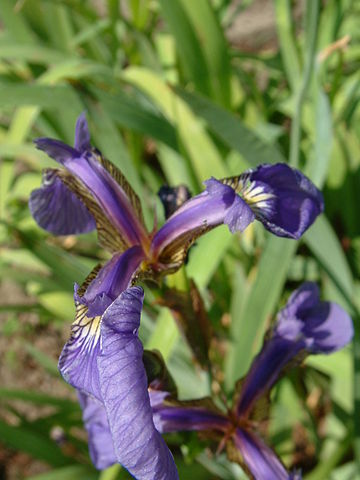
\includegraphics[height=2.5cm]{ressources/iris-setosa.jpg}&
        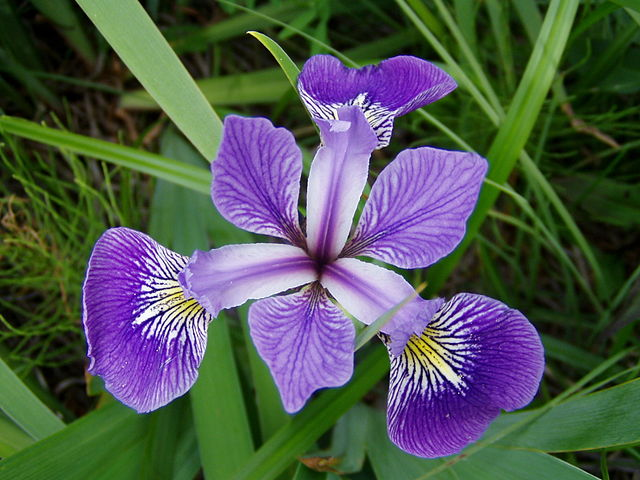
\includegraphics[height=2.5cm]{ressources/iris-versicolor.jpg}&
        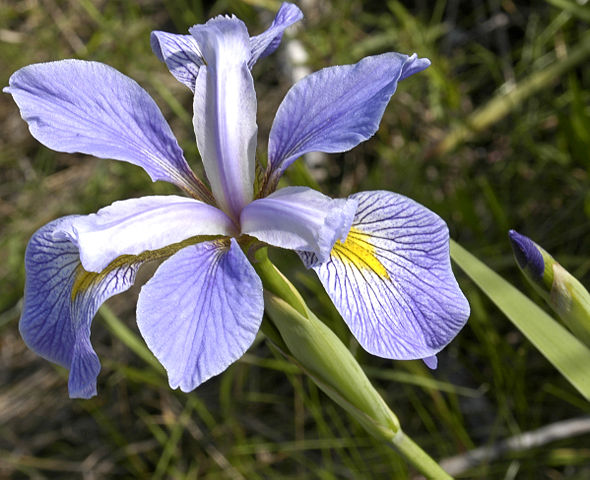
\includegraphics[height=2.5cm]{ressources/iris-virginica.jpg}\\
        Iris setosa & Iris versicolor & Iris virginica\\
    \end{tabular}
\end{center}

\end{frame}

\begin{frame}
    \frametitle{}

    \begin{center}
        \framebox{{\small Comment prédire une information nouvelle à partir de données brutes?}}
    \end{center}

\end{frame}

\section{Utiliser les données}
\subsection{Présentation graphique des informations}
\begin{frame}
    \frametitle{}

    \note[item]{Une représentation graphique des informations apporte une compréhension plus éclairante.}
    \note[item]{Il apparaît que les mesures d'un iris peuvent permettre de déterminer leur variété.}
\begin{center}
\centering
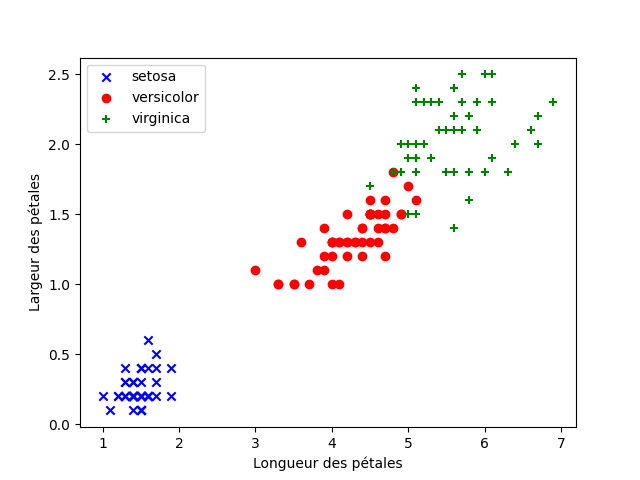
\includegraphics[width=10cm]{ressources/iris-graphe.png}
\captionof{figure}{Variétés d'iris en fonction de leurs mesures }
\label{graphe-iris}
\end{center}

\end{frame}

\subsection{Prédire la variété}
\begin{frame}
    \frametitle{Utiliser les données pour prédire}

\begin{activite}
\begin{enumerate}
    \item Déterminer la variété des iris suivants:
    \begin{tabular}{|*{5}{c|}}
        \hline
        longueur&1&6 &5.1 &2.5 \\
        \hline
        largeur&0.5&2.5& 1.55&0.85 \\
        \hline
    \end{tabular}
    \item Proposer une méthode pour effectuer un choix dans les cas ambigus.
\end{enumerate}
\end{activite}

\end{frame}

\begin{frame}
    \frametitle{Correction}
    \begin{tabular}{|*{5}{c|}}
        \hline
        longueur&1&6 &5.1 &2.5 \\
        \hline
        largeur&0.5&2.5& 1.55&0.85 \\
        \hline
        variété&setosa&virginica&ambigu&ambigu\\
        \hline
    \end{tabular}
    

\end{frame}
\section{Algorithme kNN}
\subsection{Présentation}
\begin{frame}
    \frametitle{Méthode des \textbf{k plus proches voisins}}

    Pour déterminer la variété d'un iris inconnu:
    \begin{itemize}
        \item<1-> regarder la variété d'un nombre \emph{k} de voisins,
        \begin{center}
            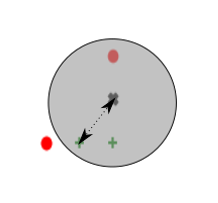
\includegraphics[width=4cm]{ressources/zoom-k3-slides.png}
        \end{center}
        \item <2-> attribuer à la fleur inconnue, la variété la plus présente parmi ses \emph{k} voisins.
    \end{itemize}
     \note{\textbf{k N}earest \textbf{N}eighbors}

\end{frame}

\begin{frame}
    \frametitle{Choix de k}

    \begin{center}
        \centering
        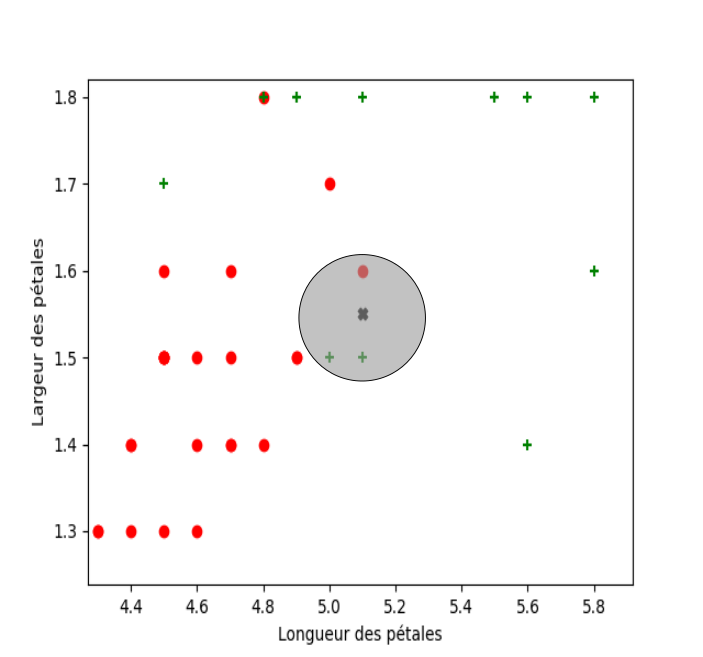
\includegraphics[width=8cm]{ressources/zoom-k3.png}
        \captionof{figure}{Détermination de l'iris (5.05, 1.5) pour $k = 3$}
        \label{IMG}
        \end{center}
\end{frame}
\begin{frame}
    \frametitle{Choix de k}

    \begin{center}
        \centering
        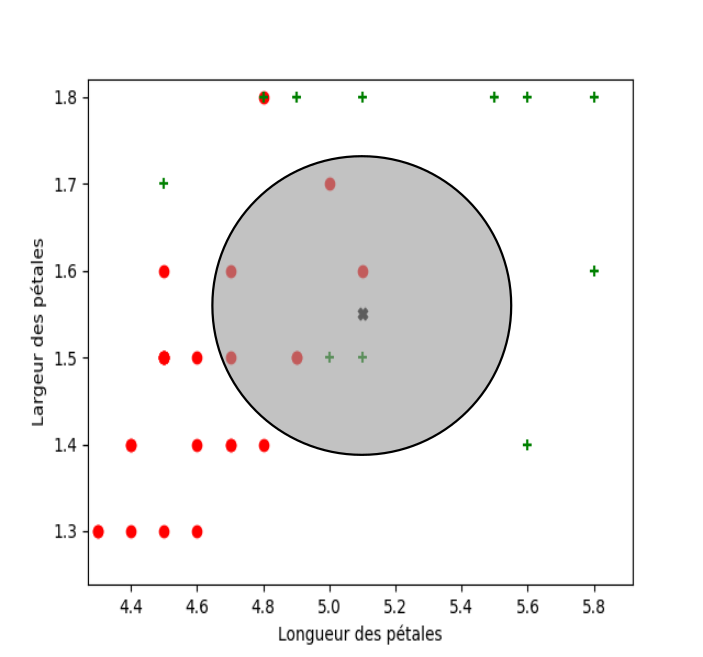
\includegraphics[width=8cm]{ressources/zoom-k7.png}
        \captionof{figure}{Détermination de l'iris (5.05, 1.5) pour $k = 7$}
        \label{IMG}
        \end{center}
        \note[item]{avantages de kNN: simple d'implémentation et résultats avec bon taux de réussite quand on a un gros échantillon}
        \note[item]{inconvénients: sensible au bruit (données mal étiquetées), sensible à l'échelle de chaque dimension}
\end{frame}

\begin{frame}
    \frametitle{}
%type d'apprentissage?
    \begin{aretenir}[Complément]
        L'algorithme \emph{kNN} est une méthode d'apprentissage \emph{supervisé}: l'algorithme reçoit un ensemble de données déjà étiquetées sur lequel il va pouvoir s’entraîner et définir un modèle de prédiction. 
        \end{aretenir}
\note[item]{non supervisé: données pas étiquetées}
\note[item]{par renforcement: par récompense}
\end{frame}

\subsection{Construction de l'algorithme}
\begin{frame}
    \frametitle{Calcul de la distance}
 Le plus naturel ici est de prendre la distance \emph{à vol d'oiseau} ou plus formellement la \textbf{distance euclidienne}.
$$d=\sqrt{(x_A-x_B)^2+(y_A-y_B)^2}$$
\begin{center}
\centering
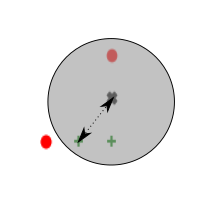
\includegraphics[width=4cm]{ressources/euclidienne.png}
\captionof{figure}{distance euclidienne}
\label{IMG}
\end{center}
\end{frame}

\begin{frame}
    \frametitle{Calcul de la distance}

$$d=\lvert x_A-x_B\rvert+\lvert y_A-y_B\rvert$$
\begin{center}
\centering
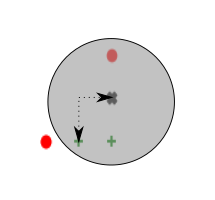
\includegraphics[width=4cm]{ressources/manhattan.png}
\captionof{figure}{distance de Manhattan}
\label{IMG}
\end{center}
\end{frame}

\begin{frame}
    \frametitle{}

    \begin{activite}
        Écrire \emph{en langage naturel}, l'algorithme kNN.
        %stocker les données
        %choisir k
        \end{activite}

\end{frame}

\begin{frame}
    \frametitle{Correction}
\begin{itemize}
    \item Charger les données dans le programme.
    \item Choisir k.
    \item Stocker les mesures de la fleur inconnue.
    \item Calculer la distance euclidienne entre la fleur inconnue et tous les autres iris.
    \item Sélectionner les \emph{k} plus proches iris (en distance) de la fleur inconnue.
    \item Affecter la variété majoritaire  des \emph{k} plus proches iris (en distance) à la fleur inconnue.
\end{itemize}
    

\end{frame}
\subsection{Implémentation}
\begin{frame}
    \frametitle{}
Pour charger les données on utilisera la bibliothèque \emph{csv}.

\end{frame}

\begin{frame}
    \frametitle{}

    \begin{activite}
        \begin{enumerate}
            \item Télécharger le dossier compressé \emph{iris.zip} sur le site \url{https://cviroulaud.github.io}
            \item Ouvrir le fichier \emph{data-iris.csv} avec un tableur pour observer les données.
            \item Ouvrir le fichier \emph{iris-eleve.py}.
            
            
        \end{enumerate}
        \end{activite}

\end{frame}
\begin{frame}
    \frametitle{Correction}

    \begin{center}
        \begin{tabular}[]{|*{3}{c|}}
            \hline
            petal\_length&petal\_width&species\\
            \hline
            1.4&0.2&setosa\\
            \hline
            1.4&0.2&setosa\\
            \hline
            1.3&0.2&setosa\\
\hline
        \end{tabular}
    \end{center}
\note{3 attributs}
\end{frame}
\begin{frame}
    \frametitle{}
    \setcounter{compteuractivite}{2}

    \begin{activite}

        \begin{enumerate}
            \setcounter{enumi}{3}

            \item Compléter la fonction \emph{charger\_donnees} en utilisant les informations du fichier \emph{csv}.
            \item Compléter la fonction \emph{distance} qui calcule le carré de la distance euclidienne entre deux points du plan.
            \item Compléter la fonction \emph{calculer\_distances}.
            \item Compléter enfin la fonction \emph{trouver\_variete}. Le dictionnaire \emph{compteur\_voisins} compte le nombre d'apparitions de chaque variété parmi les \emph{k} voisins.
        \end{enumerate}
    \end{activite}

\end{frame}
\begin{frame}
    \frametitle{Correction}

    \lstinputlisting[firstline=12 ,lastline=22, basicstyle=\small, xrightmargin=1em, xleftmargin=1em ]{"scripts/iris-correction.py"}

\end{frame}
\begin{frame}
    \frametitle{Correction}

    \lstinputlisting[firstline=25 ,lastline=26, basicstyle=\small, xrightmargin=1em, xleftmargin=1em ]{"scripts/iris-correction.py"}

\end{frame}
\begin{frame}
    \frametitle{Correction}

    \lstinputlisting[firstline=29 ,lastline=38, basicstyle=\small, xrightmargin=1em, xleftmargin=1em ]{"scripts/iris-correction.py"}

\end{frame}
\begin{frame}
    \frametitle{Correction}

    \lstinputlisting[firstline=41 ,lastline=58, basicstyle=\small, xrightmargin=1em, xleftmargin=1em ]{"scripts/iris-correction.py"}

\end{frame}
\begin{frame}
    \frametitle{}
    \setcounter{compteuractivite}{2}

    \begin{activite}

        \begin{enumerate}
            \setcounter{enumi}{7}

            \item Tester la fonction avec $k=3$ puis $k=7$, puis pour les autres iris de l'activité 1.
            \item \underline{Pour les plus avancés:} Modifier le code pour tester un ensemble de 10 iris inconnus. De plus chaque iris déterminé sera ajouté au dictionnaire \emph{varietes} afin d'augmenter l'apprentissage de l'algorithme.
        \end{enumerate}
    \end{activite}

\end{frame}
\begin{frame}
    \frametitle{Correction}

    \lstinputlisting[firstline=65 ,lastline=72, basicstyle=\small, xrightmargin=1em, xleftmargin=1em ]{"scripts/iris-correction.py"}

\end{frame}
\begin{frame}
    \frametitle{Correction}

    \lstinputlisting[firstline=77 ,lastline=88, basicstyle=\small, xrightmargin=1em, xleftmargin=1em ]{"scripts/iris-correction.py"}

\end{frame}
\end{document}